\label{sec:dispersion_cal_an_exp}
  Дисперсия возникает в том случае, когда есть спектральная расходимость источника, и
   угол Брэгга монохроматора отличается от угла Брэгга исследуемого кристалла-образца
   (рис. \ref{fig:double_crystal_schem_disp_a}).
  \begin{figure}[H]
    \centering
    \subfloat[]{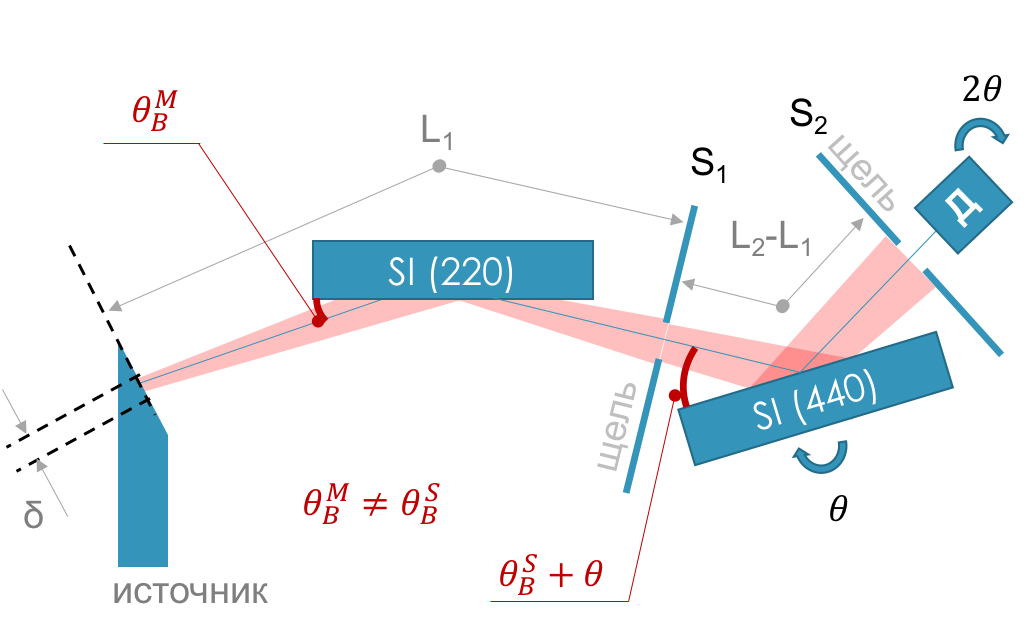
\includegraphics[width=0.6\textwidth]{images/double_crystal_schem_disp.png}\label{fig:double_crystal_schem_disp_a}}
    \hfill
    \subfloat[]{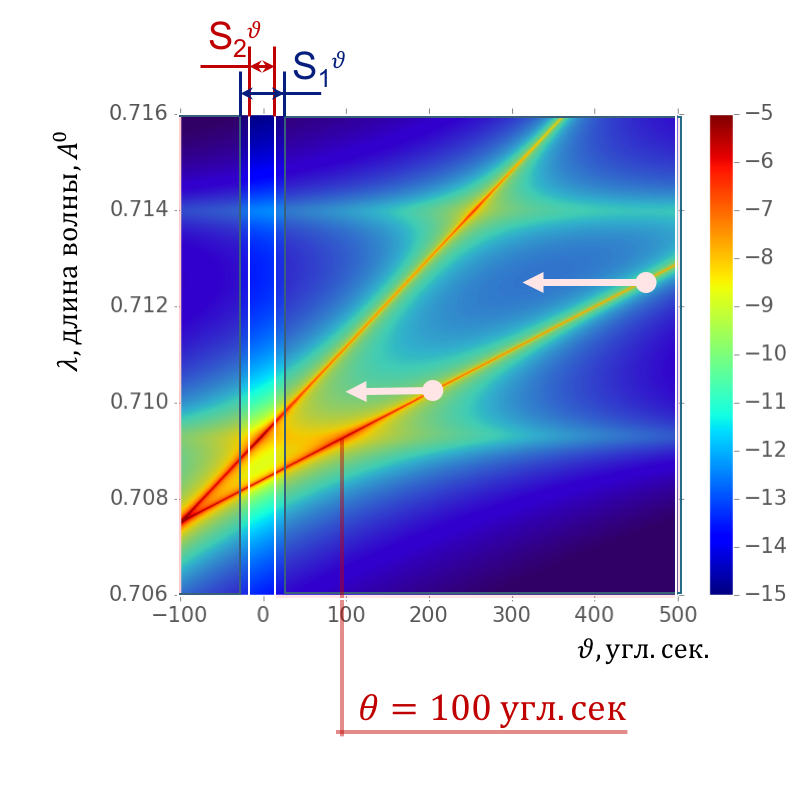
\includegraphics[width=0.35\textwidth]{images/double_crystal_lamtet_disp.png}\label{fig:double_crystal_schem_disp_b}}
    \caption{Дисперсионная схема дифракции в реальном пространстве (a) и в спектрально-угловом представлении (b)}
    \label{ris:double_crystal_schem_disp}
  \end{figure}
  Факт наличия дисперсии можно проанализировать на спектрально-угловом распределении
  (рис. \ref{fig:double_crystal_schem_disp_b}). Линия отражения образца в этом случае
  не параллельна линии отражения монохроматора, и в области, близкой к точному брэгговскому
  отражению для обоих кристаллов происходит не наложение одной полосы на другую,
  как в случае бездисперсионной схемы,
  а лишь их пересечение. Легко заметить что кривая отражения будет уширенной (рис. \ref{ris:disspersion_curves_expantheory}).
  В связи с вышесказанным можно сделать вывод, что диапазон поворота образца,
   при котором происходит эффективное отражение одновременно и от него и от монохроматора,
   значительно увеличится, что напрямую является причиной уширения КДО в дисперсионной схеме по сравнению
   с бездисперсионной.

\begin{figure}[H]
  \centering
  \subfloat[]{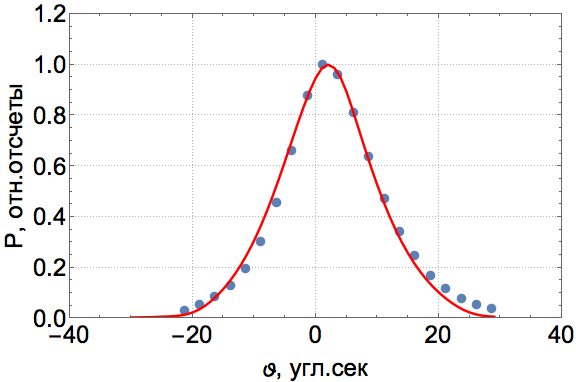
\includegraphics[width=0.45\textwidth]{images/disspers_220_440_100mcm.png}\label{fig:}}
  \hfill
  \subfloat[]{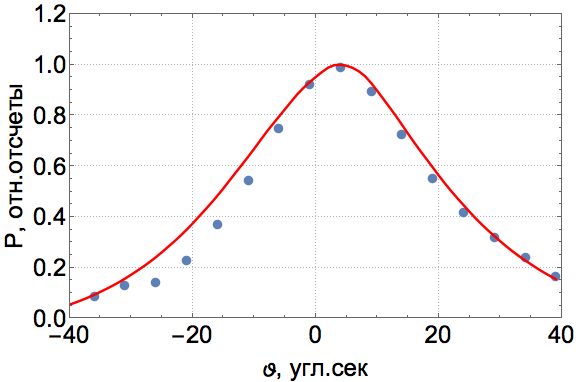
\includegraphics[width=0.45\textwidth]{images/disspers_220_660_100mcm.png}\label{fig:}}
  \hfill
  \subfloat[]{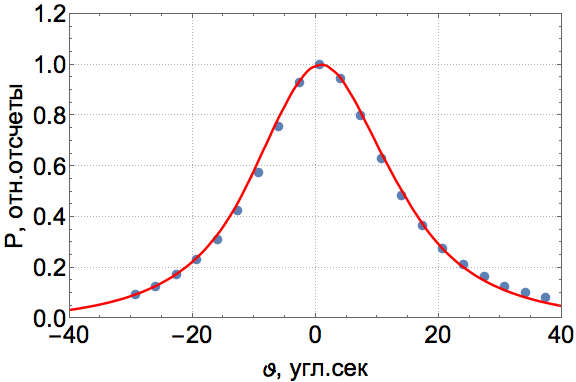
\includegraphics[width=0.45\textwidth]{images/disspers_220_440_300mcm.png}\label{fig:}}
  \hfill
  \subfloat[]{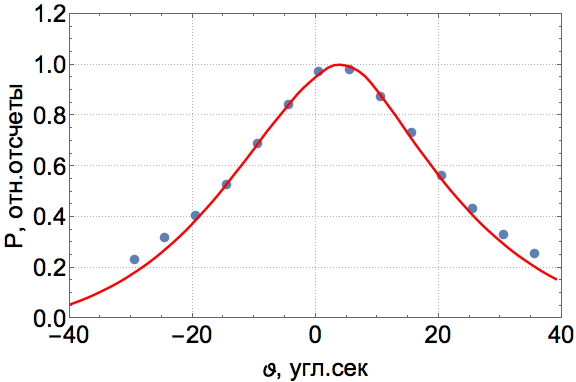
\includegraphics[width=0.45\textwidth]{images/disspers_220_660_300mcm.png}\label{fig:}}
  \caption{Двухкристальная КДО для схемы с кристаллом монохроматором Si(220) - $\theta_B = 10.6^o$
  для дисперсионного случая и разных размеров щелевых устройств:
  образец Si(440) - $\theta_B = 21.7^o$, $S_1 = S_2 = 100$ мкм (a),
   образец Si(660) - $\theta_B = 33.7^o$, $S_1 = S_2 = 100$ мкм (b),
    образец Si(440) - $\theta_B = 21.7^o$, $S_1 = S_2 = 300$ мкм (c),
     образец Si(660) - $\theta_B = 33.7^o$, $S_1 = S_2 = 300$ мкм (d)}
  \label{ris:disspersion_curves_expantheory}
\end{figure}

Дисперсия приводит к уширению КДО, величина которого может превышать полуширину собственных бездисперсионных
двухкристальных КДО в несколько раз. В дисперсионной схеме дифракции существенно заметно
влияние размера щелевых коллиматоров на полуширину КДО в отличии от бездисперсионной (см. раздел \ref{sec:non_disspers_KDO_section}).

\begin{equation}
 f_d^2 = \frac{f_S^2}{b_S}+\frac{f_M^2}{b_M}+\left( \frac{\Delta \lambda}{\lambda} (\tg(\theta_B^S) - \tg(\theta_B^M)) \right)^2.
 \label{eq:disspers_width}
\end{equation}

Так же существует формула (\ref{eq:disspers_width}) \cite{lider2009} которая выводится в приближении
гауссовской формы собственной кривой отражения от кристалла и позволяет приближенно оценить
 полуширину двухкристальных КДО с учетом дисперсии. Дисперсионное слагаемое, последнее в (\ref{eq:disspers_width})
 возникает из условия Вульфа-Брэгга. Только точный учет дисперсии позволит производить адекватный анализ собственных кривых образца.
 Безусловно, оценка дисперсионности схемы важна и при исследовании пьезоэффекта.
